% This document is compiled using pdfLaTeX
% You can switch XeLaTeX/pdfLaTeX/LaTeX/LuaLaTeX in Settings

\documentclass{article}
% \usepackage[utf8]{inputenc}
\usepackage{graphicx}
\usepackage{float}
\usepackage{amssymb}
\usepackage{amsmath}
\usepackage{graphicx}

\title{Assignment 4}
\author{221300079 Juntong Wang}
\date{\today}
    %\begin{figure}[H]
    %    \centering
    %    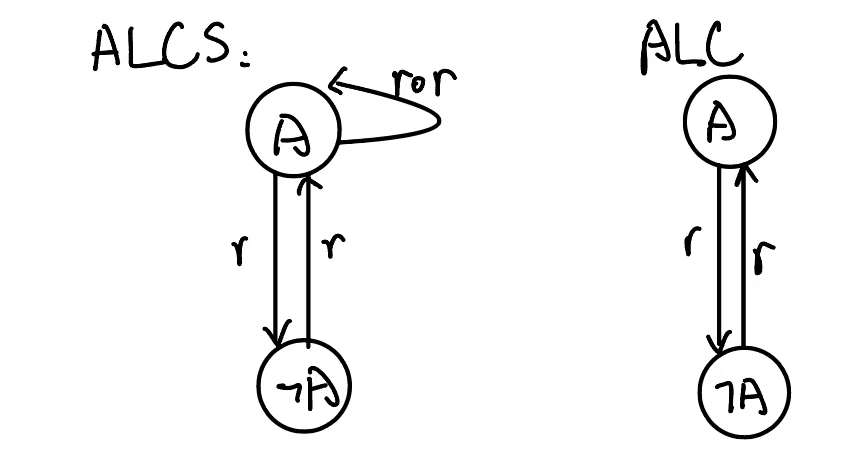
\includegraphics[width=1\textwidth]{4.png}\\
    %    \caption{Unraveling graph}
    %    \label{fig:Unraveling}
    %\end{figure}  
\newtheorem{definition}{Definition}
\setlength\parindent{0pt}

\makeatletter
\newcommand\makebig[2]{%
  \@xp\newcommand\@xp*\csname#1\endcsname{\bBigg@{#2}}%
  \@xp\newcommand\@xp*\csname#1l\endcsname{\@xp\mathopen\csname#1\endcsname}%
  \@xp\newcommand\@xp*\csname#1r\endcsname{\@xp\mathclose\csname#1\endcsname}%
}
\makeatother

\makebig{biggg} {3.0}
\makebig{Biggg} {3.5}
\makebig{bigggg}{5.0}
\makebig{Bigggg}{14.0}
\makebig{Biggggg}{20.0}
\begin{document}

	\maketitle

	\section{Question 1}
    Use the $\mathcal{ALC}$-Worlds algorithm to decide the satisfiability of the concept name $B_0$ w.r.t.\ the simple TBox:
    \begin{equation*}
    \mathcal{T}:=\Biggggl\{
    \begin{aligned} 
    B_0&\equiv B_1\sqcap B_2\\
    B_1&\equiv\exists r.B_3\\
    B_2&\equiv B_4\sqcap B_5\\
    B_3&\equiv P\\
    B_4&\equiv\exists r.B_6\\
    B_5&\equiv B_7\sqcap B_8\\
    B_6&\equiv Q\\
    B_7&\equiv\forall r.B_4\\
    B_8&\equiv\forall r.B_9\\
    B_9&\equiv\forall r.B_{10}\\
    B_{10}&\equiv\neg P
    \end{aligned}
    \Biggggl\},
    \end{equation*}
    Draw the recursion tree of a successful run and of an unsuccessful run. Does the algorithm return a positive or negative result on this input?\\
    \textbf{Here is the answer}\\
    Initial:we could get the rd of every node:
    \begin{equation*}
    \mathcal{T}:=\Bigggl\{
        \begin{aligned} 
        rd(0):B_3,B_6,B_10\\
        rd(1):B_1,B_4,B_9\\
        rd(2):B_0,B_2,B_5,B_7,B_8\\
        \end{aligned}
        \Bigggl\},
    \end{equation*}
    \textbf{Of successful run:}\\
    so the initial i is 2,and the initial $\tau = \{B_0,B_1,B_2,B_3,B_4,B_5,B_6,B_7\}$\\
    (1).$(\tau,2,T)$:for $B_1 \in\tau\ with\ B_1 \equiv\exists r.B_3$,get S = $\{B_3,B_4\}= \tau_1$;\\
    $(\tau_1,1,T)$:for $B_4 \in\tau\ with\ B_4 \equiv\exists r.B_6$,get S = $\{B_6\}= \tau_2$;\\
    $(\tau_2,0,T)$:return true;\\
    (2).$(\tau,2,T)$:for $B_4 \in\tau\ with\ B_4 \equiv\exists r.B_6$,get S = $\{B_4,B_6\}= \tau_1'$;\\
    $(\tau_1',1,T)$:for $B_4 \in\tau\ with\ B_4 \equiv\exists r.B_6$,get S = $\{B_6\}= \tau_2'$;\\
    $(\tau_2',0,T)$:return true;\\
    \textbf{Of unsuccessful run:}\\
    so the initial i is 2,and the initial $\tau = \{B_0,B_3,B_{10}\}$\\
    $(\tau,2,T)$:exists clash for the rule 1,exit,return False;\\
    Here is the representation with tree:\\
    \begin{figure}[H]
        \centering
        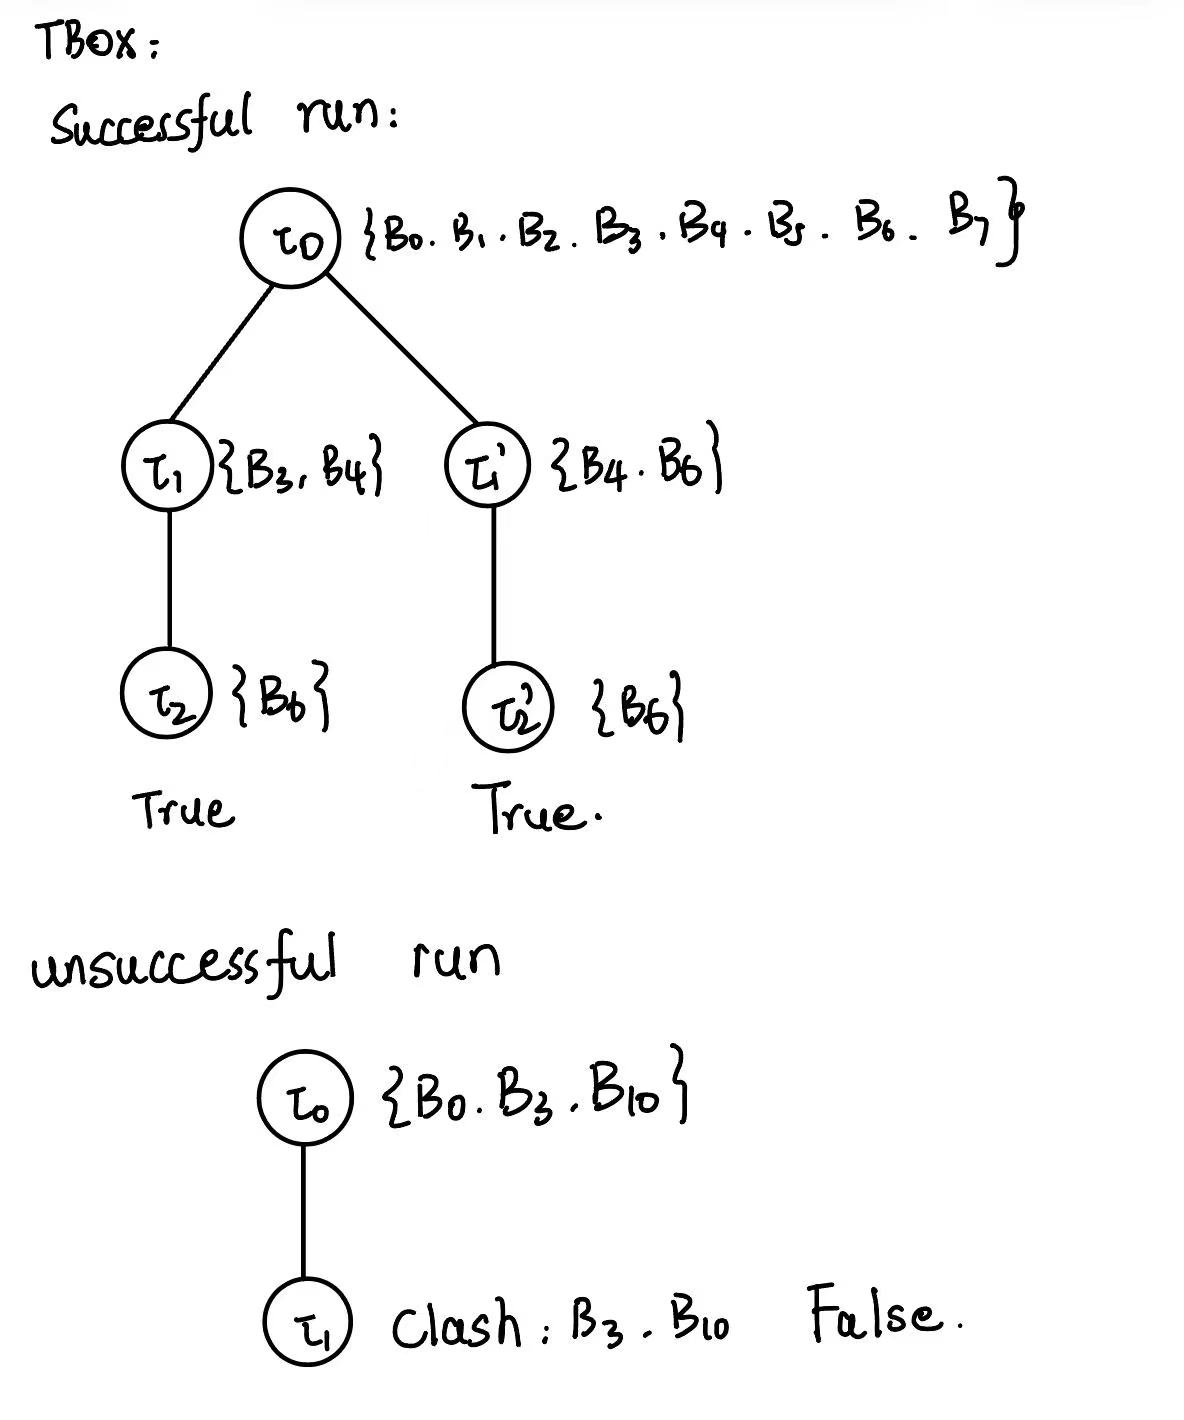
\includegraphics[width=1\textwidth]{1.png}\\
        \caption{Two ways to run the alg}
        \label{fig:Two ways to run the alg}
    \end{figure}  
    \textbf{Result:}
    There exists a successful run of the Tbox with the algorithm, so it return true, it is positive.

    \section{Question 2}
    Determine whether Player $1$ has a winning strategy in the following finite Boolean games, where in both cases $\Gamma_{1}:=\{x_1, x_3\}$ and $\Gamma_{2}:=\{x_2, x_4\}$.
    \begin{itemize}
        \item[-] $\psi :=(x_{1}\vee\neg x_{2})\wedge(x_{2}\vee x_{3})\wedge(\neg x_{3}\vee\neg x_{4})\wedge(\neg x_{1}\vee \neg x_{2}\vee x_{3}\vee x_{4})$
    \end{itemize}
    \textbf{Here is the answer:}\\
    We could get there are 4 strategies to make it true:for [x1, x2, x3, x4]\\
    $[(0, 0, 1, 0), (1, 0, 1, 0), (1, 1, 0, 1), (1, 1, 1, 0)]$ \\
    There exists no matter what the x2 choose, we could firstly choose x1, but no matter what x3 we choose the player 2 will have at least one strategy to make our loss the game.And also there is no enough leaf noeds to satisfy the need of the winning strategy.\\
    So there is no winning strategy to make the player one to win the infinite boolean game.\\

    \section{Question 3}
    Determine whether Player \textsf{2} has a winning strategy in the following infinite Boolean games where the initial configuration $t_{0}$ assigns \emph{false} to all variables.
    \begin{itemize}
        \item[-] $\psi :=(x_{1}\wedge x_{2}\wedge\neg y_{1})\vee(x_{3}\wedge x_{4}\wedge\neg y_{2})\vee(\neg(x_{1}\vee x_{4})\wedge y_{1}\wedge y_{2})$
        \item[] provided that: $\Gamma_{1}:=\{x_{1}, x_{2}, x_{3}, x_{4}\}$ and $\Gamma_{2}:=\{y_{1}, y_{2}\}$
    \end{itemize}
    \textbf{Here is the answer:}\\
    There is a winning strategy for player 1, and no winning strategy for player 2.\\
    first we get that if we could make one of the three part be true, we have the winning strategy for player one.\\
    So if the player 2 let both true, we just simple let the $\neg(x_{1}\vee x_{4})$ be true, the player 1 win.\\
    So the player 1 could do this thing, in the first two epochs, let $x_2, x_3$ be true,not to consider what the $y_1, y_2$.\\
    So if the player 2 let $y_1$ false, we just let the $x_1$ be true, so player 1 win because the $(x_{1}\wedge x_{2}\wedge\neg y_{1})$.\\
    So if the player 2 let $y_2$ false, we just let the $x_4$ be true, so player 1 win because the $(x_{3}\wedge x_{4}\wedge\neg y_{2})$.\\
    So there is a winning strategy for player 1 in this infinite boolean game.\\

    \section{Question 4}
    The universal role is a role $u$ such that its extension is fixed as $\Delta^{\mathcal{I}}\times\Delta^{\mathcal{I}}$ in any
    interpretation $\mathcal{I}$. Let $\mathcal{ALC}^{u}$ be a DL extending alc with the universal role. 
    \begin{itemize}
        \item[-] Show that concept satisfiability in $\mathcal{ALC}^{u}$ without TBoxes is EXPTIME-complete.
    \end{itemize}
    \textbf{Here is the answer:}\\
    In order to prove the $\mathcal{ALC}^{u}$ without Tboxes is also EXPTIME complete, we need to reduct it to a known EXPTIME problem. So we choose to make a reduction to the ALC with general Tbox.\\
    Then we give out proof about how to reduct then in the polynomial time.\\
    For C is the concept name, T is the general TBox,U is the concept name in $ALC^u$, we could construct the $ALC^u$ like this form:\\
    $U = C \sqcap (\forall u.(\underset{E \sqsubset F}{\sqcap} \neg E \sqcup F))$, so accroding to this form, we could translate the ALC with Tbox into $ALC^u$, so we get: C sat wrt. T iff D sat.\\
    prove:\\
    if C sat wrt.T , so we have a model I with $(\neg E \cup F)^I = \Delta^I$ where the Delta is the domain, so there must a $d_0 \in C^I, d_0 \in \Delta^I$. \\
    if D sat. So we have there is a $d_0 \in \Delta^I$, and for the universal role u:$(d_0, d)$, the d is in the $(\neg E \cup F)^I$, and we get the $d \in E^I, d\in F^I,d \in C^I$, so we have the c is sat wrt.T\\
    for this we prove that there is a way to convert the satisfiability with ALC with general Tbox into the question of $ALC^u$ without Tboxes.\\
    
    So next, we need to prove that: there is an lower bound and upper bound with the $ALC^u$ problem.\\
    
    Lower bound:\\
    As we have prove that it could be reduct to the problem of ALC with general Tbox, there is just somthing to change in the proof of general Tbox, to add the rule of universal role u.
    but actually in the proof of general Tbox, there is no change we need to do for the infinite node-labelled tree $(V,E,l)$,and the u also as the edge relation for the tree.In the same way we could prove it has 
    the lower bound of EXPTIME-hard.\\

    Upper bound:\\
    Also the same way to prove like lower bound, but there is no change for the definition 5.8, but for the definition 5.9, we redefine it like:\\
    \textbf{Redifinition of 5.9:}
    Let $\Gamma$ be a set of types and $\tau \in \Gamma$.Then $\tau$ is bad in $\Gamma$ 
    (1).if there exists an $\exists r.C\in \tau$ such that the set:
    \[
        S = \{C\}\cup \{D | \forall r.D \in \tau\}  
    \]
    is no subset of any type in $\Gamma$ and also the r is not equal to u.\\ 
    (2).if there exists an $\exists u.C\in \tau$ such that the set:$S = \{D\}$ has no subset.\\
    (3).if there exists an $\forall u,C\in \tau$ such that there is a $\tau' \in \Gamma, D \notin \tau'$.\\
    So we have the definition of bad type. And for definition 5.10, to prove the iff:\\
    (only if):$\Delta^I = \Gamma_i\\
    A^I = \{\tau \in \Gamma_i | A \in \tau\}\\
    r^I = \{(\tau,\tau')\in \Gamma_i \times \Gamma_i| \forall r.C \in \tau implies C \in \tau' \}$\\
    Then, by the induction on the structure of C, we only do the case $C = \exists u.D, C = \forall u.D$:\\
    For the case one:let $\exists r.D\in \tau$.Since $\tau$ has not been eliminated from $\Gamma_i$, it is not bad.Thus, there is 
    a $\tau'\in \Gamma_i$,such that,$\{D\}\subset \tau'$.By definition of I, we have $(\tau,\tau')\in u^I$.Since $\tau'\in C^I$ by induction hypothesis, we obtain $\tau \in(\exists u.D)^I$ by the semantics.\\
    For the case two:let $\forall r.D\in \tau$.Since $\tau$ has not been eliminated from $\Gamma_i$, it is not bad.Thus, there is 
    a $\tau'\in \Gamma_i$,such that,$\{D\}\subset \tau'$.By definition of I, we have $(\tau,\tau')\in u^I$.Since $\tau'\in C^I$ by induction hypothesis, we obtain $\tau \in(\forall u.D)^I$ by the semantics.\\
    By condition from definition 5.8, we have a model.\\
    (if):There is no need for us to change it, so remain the same as it on books.\\
    So we prove the upper bound of it is the EXPTIME-hard.\\

    All in all, there we have proved that the universal role u with $ALC^u$ without Tboxes is in EXPTIME-complete.\\
    
    \section{Question 5}
    Consider the following $\mathcal{EL}$ TBox:

    \begin{equation*}
      \mathcal{T}:=\biggggl\{
      \begin{aligned}
      A&\sqsubseteq B\sqcap\exists r.C\\
      B\sqcap\exists r.B&\sqsubseteq C\sqcap D\\
      C&\sqsubseteq(\exists r.A)\sqcap B\\
      (\exists r.\exists r.B)\sqcap D&\sqsubseteq\exists r.(A\sqcap B)
      \end{aligned}
      \biggggl\},
    \end{equation*}where $A$, $B$, $C$, $D$ are concept names. 
    
    Use the classification procedure for $\mathcal{EL}$ to check whether the following subsumptions hold w.r.t. $\mathcal{T}$.
    \begin{itemize}
    \item[-] $A\sqsubseteq\exists r.\exists r.A$
    \item[-] $B\sqcap\exists r.A\sqsubseteq\exists r.C$
    \end{itemize}
    \textbf{Here is the answer:}\\
    Firstly,we normalize the Tbox that give to us:\\
    we have:\\
    CR1:\[  \frac{}{A \sqsubseteq A}\]
    CR2:\[  \frac{}{A \sqsubseteq \top}\]
    CR3:\[  \frac{A \sqsubseteq B\ B\sqsubseteq C} {A \sqsubseteq C}\]
    CR4:\[  \frac{A\sqsubseteq B\ A\sqsubseteq C\ B\sqcap C\sqsubseteq D}{A \sqsubseteq D}\]
    CR5:\[  \frac{A\sqsubseteq \exists r.B\ B \sqsubseteq C\ \exists r.C\sqsubseteq D}{A \sqsubseteq D}\]
    (1):We could simplify the four rule it give to us and add a $A\sqsubseteq\exists r.\exists r.A$,we let 
    the $\exists r.\exists r.A \sqsubseteq L$,and we could get\\
    \begin{equation*}
        \mathcal{T}:=\Bigggggl\{
        \begin{aligned} 
        A \sqsubseteq B\\
        A \sqsubseteq \exists r.C\\
        \exists r.A \sqsubseteq M\\
        \exists r.B \sqsubseteq F\\
        \exists r.B \sqsubseteq K\\
        B \sqcap F \sqsubseteq E\\
        C \sqsubseteq \exists r.A \\
        C \sqsubseteq B\\
        E \sqsubseteq C\\
        E \sqsubseteq D\\
        H \sqsubseteq \exists r.I\\
        I \sqsubseteq A\\
        I \sqsubseteq B\\
        J \sqcap D\sqsubseteq H\\
        \exists r.K \sqsubseteq J\\
        \exists r.M \sqsubseteq L
        \end{aligned}
        \Bigggggl\},
    \end{equation*}
    And we use the CR1 to CR5 to prove the problem 1:\\
    So CR5:\[   \frac{C \sqsubseteq \exists r.A\ A\sqsubseteq A\ \exists r.A \sqsubseteq M}{C \sqsubseteq M}\]
    so CR5:\[   \frac{A \sqsubseteq \exists r.C\ C\sqsubseteq M\ \exists r.M \sqsubseteq L}{A \sqsubseteq L}\]
    So finally we find a $A\sqsubseteq L$,so it is satisfiable.\\

    (2):We could simplify the four rule it give to us and add a $B\sqcap\exists r.A\sqsubseteq\exists r.C$,
    so we get $M\sqsubseteq B\sqcap\exists r.A,\exists r.C \sqsubseteq N$,and we could get\\
    \begin{equation*}
        \mathcal{T}:=\Bigggggl\{
        \begin{aligned} 
        A \sqsubseteq B\\
        A \sqsubseteq \exists r.C\\
        \exists r.B \sqsubseteq F\\
        \exists r.B \sqsubseteq K\\
        B \sqcap F \sqsubseteq E\\
        C \sqsubseteq \exists r.A \\
        C \sqsubseteq B\\
        E \sqsubseteq C\\
        E \sqsubseteq D\\
        H \sqsubseteq \exists r.I\\
        I \sqsubseteq A\\
        I \sqsubseteq B\\
        J \sqcap D\sqsubseteq H\\
        \exists r.K \sqsubseteq J\\
        M \sqsubseteq \exists r.A\\
        M \sqsubseteq B\\
        \exists r.C \subseteq N
        \end{aligned}
        \Bigggggl\},
    \end{equation*}
    And we use the CR1 to CR5 to prove the problem 2:\\
    CR5:\[\frac{M\sqsubseteq \exists r.A\ A\sqsubseteq B\ \exists r.B \sqsubseteq F}{M\sqsubseteq F}\]
    CR5:\[\frac{A\sqsubseteq \exists r.C\ C\sqsubseteq B\ \exists r.B \sqsubseteq F}{A\sqsubseteq F}\]
    CR4:\[\frac{A\sqsubseteq B\ A\sqsubseteq F\ B\sqcap F\sqsubseteq E}{A\sqsubseteq E}\]
    CR4:\[\frac{M\sqsubseteq B\ M\sqsubseteq F\ B\sqcap F\sqsubseteq E}{M\sqsubseteq E}\]
    CR3:\[\frac{A\sqsubseteq E\ E\sqsubseteq C}{A\sqsubseteq C}\]
    CR5:\[\frac{C\sqsubseteq r.A\ A\sqsubseteq C\ \exists r.C\sqsubseteq N}{C\sqsubseteq N}\]
    CR3:\[\frac{M\sqsubseteq B\ B\sqsubseteq C}{M\sqsubseteq C}\]
    CR3:\[\frac{M\sqsubseteq C\ C\sqsubseteq N}{M\sqsubseteq N}\]
    So finally we find a $M\sqsubseteq N$,so it is satisfiable.\\

    \section{Question 6}
    Let $\mathcal{T}_{1}$ be an $\mathcal{EL}$ TBox, with $C$ and $D$ as $\mathcal{EL}$ concepts. Let us further consider $\mathcal{T}_{2}:=\mathcal{T}_{1}\cup\{A\sqsubseteq C, D\sqsubseteq B\}$, wherein $A$ and $B$ are new concept names (as in Lemma $6.1$). 
    \begin{itemize}
        \item[-] Show that $\mathcal{T}_{2}$ is a conservative extension of $\mathcal{T}_{1}$.
        \item[-] Is this still the case after adding $A\sqsubseteq B$ to $\mathcal{T}_{2}$?
        \item[-] What about adding $B\sqsubseteq A$?
    \end{itemize}
    \textbf{Here is the answer:}\\
    (1)To prove that $T_2$ is a conservative extension of $T_1$, we need to know the definition of the conservative extension.The definition said that:\\
    \begin{itemize}
        \item $sig(T_1) \subseteq sig(T_2)$
        \item every model of $T_2$ is a model of $T_1$ 
        \item for every model $I_1$ of $T_1$,there exists a model $I_2$ of $T_2$ such that the extension of concept and role names from $sig(T_1)$ coincide in $I_1$ and $I_2$,i.e:\\
            $A^{I_1} = A^{I_2}$ for all concept names $A \in sig(T_1)$ and $r^{I_1} = r^{I_2}$ for all role names $r \in sig(T_1)$\\     
    \end{itemize}
    For the first restriction,we have $T_1\ and\ T_2=T_1 \cup \{A\sqsubseteq C, D \sqsubseteq B\}$, so we could get that all signatures in $T_1$ is also in $T_2$, so the first restriction satisfied.And for the second restriction, we have lemma 2.4,we get that every model of $T_2$
    is also model of $T_1$.And for the third restriction, here we assume that $I_2$ be the interpretation that coincides with $I_1$,for A and B we could define that $A^{I_2} = C^{I_1},B^{I_2} = D^{I_1}$,so we could held that $C^{I_1} = C^{I_2},D^{I_1} = D^{I_2}$, so this yields that $A^{I_2} = C^{I_1} = C^{I_2},B^{I_2} = D^{I_1} = D^{I_2}$, so which shows that $I_2$ is also a model of$I_1$\\
    
    (2).So if we add the $A \sqsubseteq B$ to the tbox $T_2$, this indicates that there is a more restriction for the $T_2$, but accroding to the rules above, we could see that this rule has no increasing risks on the tbox $T_1$, so this will not cause the increase of the semantics as before. So this is also a conservative extension.\\
    
    (3).if we add this rule, in the interpretation $I_2$,we have that $D^{I_2} \subseteq B^{I_2} \subseteq A^{I_2} \subseteq C^{I_2}$, so here we have a expand of the semantics before. This is contradict to the definition of the conservative extension.\\

    \section{Question 7}
    We consider the DL $\mathcal{EL}_{\textsf{si}}$ extending $\mathcal{EL}$ by concept descriptions of the form $\exists^{\textsf{sim}}(\mathcal{I},\textsf{d})$, where $\mathcal{I}$ is a finite interpretation and $\textsf{d}\in\Delta^{\mathcal{I}}$. Their semantics is defined as follows.
    \[(\exists^{\textsf{sim}}(\mathcal{I},\textsf{d}))^{\mathcal{J}}:=\{\textsf{d}^{\prime}~|~\textsf{d}^{\prime}\in\Delta^{\mathcal{J}}~\text{and}~(\mathcal{I},\textsf{d})\eqsim(\mathcal{J},\textsf{d}^{\prime})\}\]
    Concept inclusions are then defined as usual.
    \begin{itemize}
        \item[-] Show that each $\mathcal{EL}_\textsf{si}$ concept description is equivalent to some concept descriptions of the form $\exists^{\textsf{sim}}(\mathcal{I},\textsf{d})$.
        \item[-] Show that $\mathcal{EL}_\textsf{si}$ is more expressive than $\mathcal{EL}$.
        \item[-] Show that checking subsumption in $\mathcal{EL}_\textsf{si}$ without any TBox can be done in polynomial time.
    \end{itemize}
    \textbf{Here is the answer:}\\
    Before giving the solution of this problem. we give out the definition of the eqsim and $\mathcal{EL}_{\textsf{si}}$.\\
    For the eqsim:Given interpretations $\mathcal{I}$ and $\mathcal{J}$, the relation $\sigma\in\Delta^{\mathcal{I}}\times\Delta^{\mathcal{J}}$ is a simulation from $\mathcal{I}$ to $\mathcal{J}$ if\\
    \begin{itemize}
        \item[$\bullet$] whenever $\textsf{d}~\sigma~\textsf{d}^{\prime}$ and $\textsf{d}\in A^{\mathcal{I}}$, then $\textsf{d}^{\prime}\in A^{\mathcal{J}}$, for all $\textsf{d}\in\Delta^{\mathcal{I}}$, $\textsf{d}^{\prime}\in\Delta^{\mathcal{J}}$, and $A\in\mathbb{C}$;
        \item[$\bullet$] whenever $\textsf{d}~\sigma~\textsf{d}^{\prime}$ and $(\textsf{d},\textsf{e})\in r^{\mathcal{I}}$, then there exists an $\textsf{e}^{\prime}\in\Delta^{\mathcal{J}}$ such that $\textsf{e}~\sigma~\textsf{e}^{\prime}$ and $(\textsf{d}^{\prime},\textsf{e}^{\prime})\in r^{\mathcal{J}}$, for all $\textsf{d},\textsf{e}\in\Delta^{\mathcal{I}}$, $\textsf{d}^{\prime}\in\Delta^{\mathcal{J}}$, and $r\in\mathbb{R}$.
    \end{itemize}
    We write $(\mathcal{I},\textsf{d})\eqsim(\mathcal{J},\textsf{d}^{\prime})$ if there is a simulation $\sigma$ from $\mathcal{I}$ to $\mathcal{J}$ such that $\textsf{d}~\sigma~\textsf{d}^{\prime}$.\\
    And then for the $\mathcal{EL}$ language, it contains exists, and, top.and for the $\mathcal{EL}_\textsf{si}$ language, accroding to the problem's description, we add another rule called $\mathcal{EL}$ by concept descriptions of the form $\exists^{\textsf{sim}}(\mathcal{I},\textsf{d})$, which could be interpreted as a simulation from I to J.\\
    
    (1).To prove that all concept descriptions in $\mathcal{EL}_\textsf{si}$ could be convert into the from of $\exists^{\textsf{sim}}(\mathcal{I},\textsf{d})$.So we construct a simulation to prove it.For an interpretation I and an interpretation J, we have a defined simulation as the problem said.So:\\
    1.For rule $C \sqcup D$, we let there is an element c could be interpret as $(C\sqcup D)^I=c^I$ with interpretation I, so accroding to the simulation $\sigma$ that could be as $c'^J \in \Delta^J$,so as the same all elements in the $C^I,D^I$, we could have the same $C^J,D^J$.So this proved could be convert.\\
    2.For rule $\top$,easily to see that $d^I\in \Delta^I$ could with the exists-sim rule given in problem be converted to the $d^J\in \Delta^J$.\\
    3.For rule $\exists r.C$, we could get $\{d|\exists e:(d,e)\in r^I\ and\ e\in C^I\}$,the same, we use the simulation to convert it to as $\{d|\exists e:(d,e)\in r^J\ and\ e\in C^J\}$.
    So all the form if  $\mathcal{EL}_\textsf{si}$ could be convert to the form as $\exists^{\textsf{sim}}(\mathcal{I},\textsf{d})$. So we proved that they equal to some concept descriptions in this form.\\  
    
    (2).To prove the $\mathcal{EL}_\textsf{si}$ is more expressive than $\mathcal{EL}$, we need to give out a situation that could be dealt in $\mathcal{EL}_\textsf{si}$ but not in  $\mathcal{EL}$. Here if we have two interpretations I and J.we have domain in two interpretations as:
    $\Delta^I = \{a,b\}$,and $\Delta^J = \{a,b,c\}$. So accroding to the definition of simulation, it is a kind of one-side bisimulations, so we could have this in I:$C^I=\{a,b\},D^I = \{a\},(C\cup D)^I = \{a\}$, but with the simulation could be this in J:$C^J=\{a,b,c\},D^J = \{a,b\},(C\cup D)^I = \{a,b\}$.Here
    the answer in I is a subset of J, so the $\mathcal{EL}_\textsf{si}$ is more expressive than $\mathcal{EL}$\\
    
    (3).To prove the $\mathcal{EL}_\textsf{si}$  is in polynomial time, we could do some reduction to it, so if the $\mathcal{EL}_\textsf{si}$ could be reducted into $\mathcal{EL}$, it is in polynomial time.
    To prove how to convert the $\mathcal{EL}$ into $\mathcal{EL}_\textsf{si}$  in polynomial time. The problem had given out a method to convert in linear time.the simulation operation is in linear time. And if we get the size of domain in
    $\Delta^I$ with n,we could assume the simulation also the $\Delta^J$ will not bigger than $n^2$, so it is also in polynomial time. Thus we reduct it to the complexity of $\mathcal{EL}$, so it without any Tbox could be down in polynomial time. 

    \section{Question 8}
    Use the $\mathcal{ALC}$-Elim algorithm to decide satisfiability of:
    \begin{itemize}
        \item[-] the concept name $A$ w.r.t.\ $\mathcal{T}:=\{A\sqsubseteq\exists r.A, \top\sqsubseteq A, \forall r.A\sqsubseteq\exists r.A\}$
        \item[-] the concept description $\forall r.\forall r.\neg B$ w.r.t.\ $\mathcal{T}:=\{\neg A\sqsubseteq B, A\sqsubseteq\neg B, \top\sqsubseteq\neg\forall r.A\}$
    \end{itemize}
    Give the constructed type sequence $\Gamma_{0}$, $\Gamma_{1},\ldots$. In the case of satisfiability, also give the satisfying model constructed in the proof of Lemma $5.10$.\\
    \textbf{Here is the answer:}\\
    For the item 1:\\
    Firstly, we get the T:$\mathcal{T}:=\{A\sqsubseteq\exists r.A, \top\sqsubseteq A, \forall r.A\sqsubseteq\exists r.A\}$\\
    so,then accroding to the general Tboxes in book, we have $C_T = \{(\neg A\sqcup \exists r.A) \sqcap A \sqcap (\exists r.\neg A \sqcup \exists r. A)\}$\\
    because the operation cap and cup will not influence the order of the whole sequence, we could add some () like this:$C_T = \{((\neg A\sqcup \exists r.A) \sqcap A )\sqcap (\exists r.\neg A \sqcup \exists r. A)\}$ or $C_T = \{(\neg A\sqcup \exists r.A) \sqcap (A \sqcap (\exists r.\neg A \sqcup \exists r. A))\}$,
    and we choose the first form to make the subset more easy.\\
    then we get sub(T)=$\{A,\neg A,\exists r.A,\exists r.\neg A,(\neg A \sqcup \exists r.A), (\exists r. \neg A \sqcup \exists r.A), ((\neg A \sqcup \exists r.A) \sqcap A),((\neg A\sqcup \exists r.A) \sqcap A )\sqcap (\exists r.\neg A \sqcup \exists r. A)\}$\\
    So through the type operation, we get:\\
    $\mathcal{T} = \{A,\exists r.A,(\neg A \sqcup \exists r.A), (\exists r. \neg A \sqcup \exists r.A), ((\neg A \sqcup \exists r.A) \sqcap A),((\neg A\sqcup \exists r.A) \sqcap A )\sqcap (\exists r.\neg A \sqcup \exists r. A) \},\\
        \{A, \exists r.A,\exists r.\neg A,(\neg A \sqcup \exists r.A), (\exists r. \neg A \sqcup \exists r.A), ((\neg A \sqcup \exists r.A) \sqcap A),((\neg A\sqcup \exists r.A) \sqcap A )\sqcap (\exists r.\neg A \sqcup \exists r. A)\}$\\
    So we do the first time of elim algorithm, and we get that:in the second part, there is no $\neg A$ subset, so it is bad, so the $\mathcal{T}_1$ could be:\\
    $\mathcal{T}_1 = \{A,\exists r.A,(\neg A \sqcup \exists r.A), (\exists r. \neg A \sqcup \exists r.A), ((\neg A \sqcup \exists r.A) \sqcap A),((\neg A\sqcup \exists r.A) \sqcap A )\sqcap (\exists r.\neg A \sqcup \exists r. A) \}$\\
    And go on, the $\mathcal{T}_1$ could be:\\
    $\mathcal{T}_2 = \{A,\exists r.A,(\neg A \sqcup \exists r.A), (\exists r. \neg A \sqcup \exists r.A), ((\neg A \sqcup \exists r.A) \sqcap A),((\neg A\sqcup \exists r.A) \sqcap A )\sqcap (\exists r.\neg A \sqcup \exists r. A) \}$\\
    And we get $\mathcal{T}_1$ =$\mathcal{T}_2$, reach the end condition of elim.So this is the answer.
    So the model is :
    $\mathcal{T}_{model} = \{A,\exists r.A,(\neg A \sqcup \exists r.A), (\exists r. \neg A \sqcup \exists r.A), ((\neg A \sqcup \exists r.A) \sqcap A),((\neg A\sqcup \exists r.A) \sqcap A )\sqcap (\exists r.\neg A \sqcup \exists r. A) \}$\\
    So B is satisfiable.\\

    For the item 2:\\
    accroding to the description of 5.1.2 in general tbox,firstly we introduce the compound concept into the Tbox as the form $A_0\sqsubseteq \forall r.\forall r.\neg B$.So do nnf
    to the Tbox, we get:\\
    The box:$\top \sqsubseteq \{(A\sqcup B)\sqcap (\neg A \sqcup \neg B)\sqcap (\exists r.\neg A)\sqcap (\neg A_0 \sqcup \forall r.\forall r.\neg B)\}$\\
    So we could get the sub:$\{A,\neg A,B,\neg B,A_0,\neg A_0,\forall r.\forall r.\neg B,\forall r.\neg B,\exists r.\neg A, 
    (A\sqcup B), (\neg A \sqcup \neg B),(\exists r.\neg A), (\neg A_0 \sqcup \forall r.\forall r.\neg B),
    (\neg A_0 \sqcup \forall r.\forall r.\neg B)\sqcap (A\sqcup B),
    (\neg A_0 \sqcup \forall r.\forall r.\neg B)\sqcap (A\sqcup B)\sqcap (\neg A \sqcup \neg B),
    (\neg A_0 \sqcup \forall r.\forall r.\neg B)\sqcap (A\sqcup B)\sqcap (\neg A \sqcup \neg B)\sqcap  (\neg A_0 \sqcup \forall r.\forall r.\neg B)\}$\\
    To simplify the sentence,we could know from definition 5.8 that we let the $C_T$ be the $\{(A\sqcup B), (\neg A \sqcup \neg B),(\exists r.\neg A), (\neg A_0 \sqcup \forall r.\forall r.\neg B),
    (\neg A_0 \sqcup \forall r.\forall r.\neg B)\sqcap (A\sqcup B),
    (\neg A_0 \sqcup \forall r.\forall r.\neg B)\sqcap (A\sqcup B)\sqcap (\neg A \sqcup \neg B),
    (\neg A_0 \sqcup \forall r.\forall r.\neg B)\sqcap (A\sqcup B)\sqcap (\neg A \sqcup \neg B)\sqcap  (\neg A_0 \sqcup \forall r.\forall r.\neg B)\}$,because it doesn't contains single element so every subset includes them.\\
    So we get $\mathcal{T}$ as follow:\\
    1.$\{C_T,\neg A, B, \forall r.\forall r.\neg B\}$\\
    2.$\{C_T,\neg A, B, \forall r.\forall r.\neg B, \forall r.\neg B\}$\\
    3.$\{C_T,\neg A, B, A_0, \forall r.\forall r.\neg B\}$\\
    4.$\{C_T,\neg A, B, A_0, \forall r.\forall r.\neg B,\forall r.\neg B\}$\\
    5.$\{C_T,\neg A, B, \neg A_0\}$\\
    6.$\{C_T,\neg A, B, \neg A_0, \forall r.\neg B\}$\\
    7.$\{C_T,\neg A, B, \neg A_0, \forall r.\forall r.\neg B\}$\\
    8.$\{C_T,\neg A, B, \neg A_0, \forall r.\neg B,\forall r.\forall r.\neg B\}$\\
    9.$\{C_T, A,\neg B, \forall r.\forall r.\neg B\}$\\
    10.$\{C_T, A,\neg B, \forall r.\forall r.\neg B, \forall r.\neg B\}$\\
    11.$\{C_T, A,\neg B, A_0, \forall r.\forall r.\neg B\}$\\
    12.$\{C_T, A,\neg B, A_0, \forall r.\forall r.\neg B,\forall r.\neg B\}$\\
    13.$\{C_T, A,\neg B, \neg A_0\}$\\
    14.$\{C_T, A,\neg B, \neg A_0, \forall r.\neg B\}$\\
    15.$\{C_T, A,\neg B, \neg A_0, \forall r.\forall r.\neg B\}$\\
    16.$\{C_T, A,\neg B, \neg A_0, \forall r.\neg B,\forall r.\forall r.\neg B\}$\\
    In these, we could get that all the odd (the start is 1),could get into nect epoch.\\
    So we get $\mathcal{T}_1$ as follow:\\
    1.$\{C_T,\neg A, B, \forall r.\neg B\}$\\
    3.$\{C_T,\neg A, B, A_0, \forall r.\neg B\}$\\
    5.$\{C_T,\neg A, B, \neg A_0\}$\\
    7.$\{C_T,\neg A, B, \neg A_0, \forall r.\neg B\}$\\
    9.$\{C_T, A,\neg B, \forall r.\neg B\}$\\
    11.$\{C_T, A,\neg B, A_0, \forall r.\neg B\}$\\
    13.$\{C_T, A,\neg B, \neg A_0\}$\\
    15.$\{C_T, A,\neg B, \neg A_0, \forall r.\neg B\}$\\
    In these, we could get that only 5 and 13,could get into nect epoch.\\
    So we get $\mathcal{T}_2$ as follow:\\
    5.$\{C_T,\neg A, B, \neg A_0\}$\\
    13.$\{C_T, A,\neg B, \neg A_0\}$\\
    So actually this is unstatisfiable,so return false.

    \section{Question 9}
    We consider simulations, which are ``one-sided'' variants of bisimulations. Given interpretations $\mathcal{I}$ and $\mathcal{J}$, the relation $\sigma\in\Delta^{\mathcal{I}}\times\Delta^{\mathcal{J}}$ is a simulation from $\mathcal{I}$ to $\mathcal{J}$ if
    \begin{itemize}
        \item[$\bullet$] whenever $\textsf{d}~\sigma~\textsf{d}^{\prime}$ and $\textsf{d}\in A^{\mathcal{I}}$, then $\textsf{d}^{\prime}\in A^{\mathcal{J}}$, for all $\textsf{d}\in\Delta^{\mathcal{I}}$, $\textsf{d}^{\prime}\in\Delta^{\mathcal{J}}$, and $A\in\mathbb{C}$;
        \item[$\bullet$] whenever $\textsf{d}~\sigma~\textsf{d}^{\prime}$ and $(\textsf{d},\textsf{e})\in r^{\mathcal{I}}$, then there exists an $\textsf{e}^{\prime}\in\Delta^{\mathcal{J}}$ such that $\textsf{e}~\sigma~\textsf{e}^{\prime}$ and $(\textsf{d}^{\prime},\textsf{e}^{\prime})\in r^{\mathcal{J}}$, for all $\textsf{d},\textsf{e}\in\Delta^{\mathcal{I}}$, $\textsf{d}^{\prime}\in\Delta^{\mathcal{J}}$, and $r\in\mathbb{R}$.
    \end{itemize}
    We write $(\mathcal{I},\textsf{d})\eqsim(\mathcal{J},\textsf{d}^{\prime})$ if there is a simulation $\sigma$ from $\mathcal{I}$ to $\mathcal{J}$ such that $\textsf{d}~\sigma~\textsf{d}^{\prime}$.
    \begin{itemize}
        \item[-] Show that $(\mathcal{I},\textsf{d})\sim(\mathcal{J},\textsf{d}^{\prime})$ implies $(\mathcal{I},\textsf{d})\eqsim(\mathcal{J},\textsf{d}^{\prime})$ and $(\mathcal{J},\textsf{d}^{\prime})\eqsim(\mathcal{I},\textsf{d})$.
        \item[-] Is the converse of the implication above also true?
        \item[-] Show that, if $(\mathcal{I},\textsf{d})\eqsim(\mathcal{J},\textsf{d}^{\prime})$, then $\textsf{d}\in C^{\mathcal{I}}$ implies $\textsf{d}^{\prime}\in C^{\mathcal{J}}$ for all $\mathcal{EL}$ concept descriptions $C$.
        \item[-] Which of the constructors disjunction, negation, or universal restriction can be added to $\mathcal{EL}$ without losing the property above?
        \item[-] Show that $\mathcal{ALC}$ is more expressive than $\mathcal{EL}$.
    \end{itemize}
    \textbf{Here is the answer:}\\
    (1).Firstly we give out the definition of bisimulations.Let there are two interpretations I and J, we have $\rho \subseteq \Delta^I \times \Delta^J$:\\
    1.$d_1\ \rho\ d_2$ implies $d_1 \in A^I\ iff\ d_2 \in A^J$ for all A$\in C$\\
    2.$d_1\ \rho\ d_2$ and $(d_1,d_1')\in r^I$ implies the existence of $d_2'\in \Delta^J$ such that $d_1'\ \rho\ d_2'$ and $(d_2,d_2')\in r^J$ for all $r\in \mathcal{R}$\\
    3.$d_1\ \rho\ d_2$ and $(d_2,d_2')\in r^I$ implies the existence of $d_1'\in \Delta^J$ such that $d_1'\ \rho\ d_2'$ and $(d_1,d_1')\in r^J$ for all $r\in \mathcal{R}$\\
    So easily we could find that the definition in bisimulation 1 and 2 is equal to simulation $(\mathcal{I},\textsf{d})\eqsim(\mathcal{J},\textsf{d}^{\prime})$, and the definition of bisimulation 1 and 3 equal to simulation $(\mathcal{J},\textsf{d})\eqsim(\mathcal{I},\textsf{d}^{\prime})$, so this proved that
    $(\mathcal{I},\textsf{d})\sim(\mathcal{J},\textsf{d}^{\prime})$ implies $(\mathcal{I},\textsf{d})\eqsim(\mathcal{J},\textsf{d}^{\prime})$ and $(\mathcal{J},\textsf{d}^{\prime})\eqsim(\mathcal{I},\textsf{d})$.\\

    (2).The converse of the implication above is not true.Because the simulation is kind of one side of bisimulations.What in bisimulations restrict that the role and concept name are one to one mapping.Here the simulation could map from one element like $d^I\in \Delta^I$ to maybe a lot elements in the $\Delta^J$.
    So if converse, the mapping relationship is not true for th  em.\\

    (3)if $(\mathcal{I},\textsf{d})\eqsim(\mathcal{J},\textsf{d}^{\prime})$,we need to prove that for all rules in  $\mathcal{EL}$ is also true.\\
    So we use the constructive inductions.\\
    1.for rule $C\sqcup D$,we let under the interpretation I could as $(C\cup D)^I = \{a\}$, so by the definition of simulation,for all element in $c\in C^I$, we have $c \rho c'$, then $c'\in D^J$.And this also helds for D,so as the rule $(C \cup D)^I$ could also be translated into $(C\cup D)^J = \{c'\}$.\\
    2.for rule top,this is easily see if I and J have simulation relationship, we get the top for the same.\\
    3.for rule exists, if $\exists r.C$ could be interpret in I as $d\in \Delta^I,(d,d')\in r^I\ and\ d' \in C^I$,by the definition of simulation, this could be as
    $e\in \Delta^J,(e,e')\in r^J\ and\ e' \in C^J$ with interpretation J, so the exist rule is also satisfiable.\\
    By do simulation on $\mathcal{EL}$ above, we proved that the problem item 3 holds.\\

    (4).To prove that which constructor could be added to $\mathcal{EL}$ without losing the property,we do some analyse.\\
    1.for operator disjunction, we let two interpretation I and J that under interpretation I, the $(C \cap D)^I$ could be interpreted as $\{a,b\}\in \Delta^I$,so as the same prove way of conjunction, we could also get 
    this holds in $(C\cap D)^J$ in $\Delta^J$. And if we added this operator to $\mathcal{EL}$, this will not change the property above. \\
    2.for operator negation, this couldn't be added. We konw that the ALC = $FL_0$ + EL, but with the operator of negation, it extends the semantics to ALC but not EL, so lose the property in EL.\\
    3.for operator u as universal restriction, this is a valid operator in language $FL$, and $FL_0$ is a subset of $FL$, so this is not valid in $\mathcal{EL}$.
    In all, we could added disjunction to it without change its property.\\
    
    (5)To prove it more expressive, we construct an example:\\
    If we use the negation in ALC to solve problems, here we only need $\neg,\cap,\exists$ there 3 operators that could descript all the symbols
    in the ALC concepts $\neg,\cup,\cap,\forall,\exists$.But actually there is no operators in EL that could get the meaning of $\forall,\cup,\neg$, so ALC
    is definitly more expressive than what EL done.


\end{document}


